\chapter{導論}
\section{研究動機}
  
語言是人與人彼此交流最主要的橋樑,而人們互相溝通最自然的方式便是透過說話的語音(Speech)達成。人類往往是自幼就牙牙學語開始說話,直到已屆學齡左右才開始學習認字與書寫。雖然在這個資訊爆炸的時代,人們已經習慣以文字呈現的語言作為獲取資訊的主要媒介,但不論如何,各種書寫系統其背後承載的語言必定有語音的形式作為對應。更何況世界上現存大約七千多種 \cite{eberhard_ethnologue_2024} 語言中,絕大多數不見得存在成熟且普及的文字系統,卻無礙於這些語言被人們所熟悉和使用。因此,「語音」作為語言不可或缺的存在方式,了解它和研究它的價值自然不言而喻。

然而,相對於穩定、易於處理和保存的文字文本,語音訊號的變化萬千,蘊藏了大量從語者風格、表達內容到抑揚頓挫(韻律,Prosody)等不同層次的訊息,使得對它的處理、研究相比之下複雜度與難度劇增。由於語音的這種特性,過往對於語言最有興趣的語言學家們,即便明白語音作為多數語言主體的事實,也不得不藉文字符號為依託進行探索。進入資訊化時代後,藉助電腦硬體等計算設備的幫助,從語料庫、計算語言學到自然語言處理等透過科技的力量發展語言處理技術的領域,頗長一段時間也是專注於文字的處理與分析。
而嘗試結合訊號處理發展的語音技術領域,當時則是透過語言學家對語言的領域知識,例如從音位(Phoneme)、構詞(Morphology)、語法(Syntax)等等用以刻劃人類語音和語言特性的概念,將之結合機器學習建立模型,開發技術以方便人們能以語音這種更靈活的媒介,更好的讓電腦、手機等科技工具可以更接近「直接溝通」的使用方式,便利人們的日常生活。

近年來,由於圖形處理器(Graphics Processing Unit,GPU)等硬體平行運算技術的進步,深層學習(Deep Learning)快速崛起成為人工智慧的主流,有了此項機器學習的技術,模型的彈性能夠更好的萃取資料、更貼近的尋找資料背後的機制並進行預測,使得人們不再非得依賴大量費時費工的人類標注過程,進而使得利用大量語料庫發展語言技術,進一步推進語言科技發展成為可能。尤其在自監督學習(Self-supervised Learning)技術出現之後,深層學習模型可以依照人們給定的方向,更細緻的從大量未標注、相較容易取得的語音或文字的語料,找出其中的語音、語法及語義等等結構,形成帶有對人類語言有前所未見表現的基石模型(Foundation Model),是這個領域的一大里程碑。尤其在以處理文字為主體的自然語言處理領域,甚至出現了幾乎使人類真偽難辨的生成式模型,改變了人們生活的方方面面。

借鏡文字方面的成功經驗,語音處理領域的研究者們也開始嘗試將語言模型(Language Model)的概念套用於變化莫測的語音訊號之上,原先人們藉助訊號處理知識一直使用的各種語音訊號特徵(Feature)也在自監督學習的架構之下,出現了許多模型從大量語音資料中得到的「語音表徵(Speech Representation)」,作為精煉語音資訊的另外一種新選擇開始廣泛被採用。然而,相比於文字符號的穩定與單純,語音的複雜性使得它處理起來會需要更大量的資料和運算資源來擷取其中不同層次的細節,而且作為物理訊號,語音還必須處理掉環境中的雜訊等干擾。為了從紛亂的聲音中提取出最重要的訊息,向量量化(Vector Quantization)的技巧因而經常被使用在語音 \cite{chorowski_unsupervised_2019,chen_vector_2023,zhao_speech_2023} 或影像的領域中。爾後, \cite{lakhotia_generative_2021-1}  基於模仿人類學習語言的過程,藉助諸如 CPC(\cite{oord_representation_2019} )、HuBERT (\cite{hsu_hubert_2021} )、wav2vec 2.0 (\cite{baevski_wav2vec_2020} )等自監督學習模型的幫助,引入向量量化的技術,提出了「無文字(Textless)」的學習架構,轉而以語音表徵量化後的「離散單元(Discrete Unit)」作為操作對象,企圖以單純大量的語音資料中訓練出一個不依賴文字的語言模型。此種學習架構的優勢在於在能保有利用大量未標注文字轉寫語音資料的同時,與連續表徵相比資訊的位元率(Bit Rate)利用更有效率、容易儲存、處理與傳輸,以及形式上更像文字的特性,因而可以將其視為一種「機器自己學習出來的文字」,接下來借用長久以來只能在自然語言處理(Natural Language Processing,NLP)領域中各種語言模型(Language Model)的相關技術和任務的解決方法,套用在語音處理的領域中,期望可以像文字那樣從大量的語音資料中,找尋出「語音訊號版本的文字」。自此之後有一系列如應用於英語和閩南語之間的語音到語音翻譯 \cite{chen_speech--speech_2023} 等等使用離散單元(Discrete Unit)進行任務訓練的研究,一定程度的印證了這些離散單元捕捉語音內容的效果。

儘管離散單元在編碼語音之上固然有不錯的效果,並有相關研究展現了離散單元具有一定程度上與文字的相似性,然而其作為「完全文字的替代」仍然有相當的距離。借鑑過往在自監督學習的語音表徵出來之後,便嘗試重新從語言學(Linguistics)的概念汲取靈感,對其進行語音學(Phonetics)層面的分析。本論文期望初步結合原先 HuBERT 中從消息理論(Information Theory)的統計數據,結合語音學分析的視角,對於離散表徵(Discrete Representation)本身與音位(Phoneme)和語音類別(Phone Type)之間的關係進行相關性的統計與分析,期望可以對 HuBERT 等自監督學習表徵進行量化(Quantization)後所得的離散單元所編碼、擷取到的資訊是什麼有較為深入程度的了解。


% 直接快速帶過連續的 Speech Repr
% Acoustic Piece 那邊的文獻到後面再寫。到這裡已經夠承先啟後了
    
\section{研究方向}
  
本研究論文為了探究離散單元本身是否具有潛力可以單純透過大量語音資料的自監督學習與統計過程,從文本中找尋出語音中更精細的結構,乃至於類似文字或是從語言學(Linguistics)等人類知識領域定義出的「離散單位」 --- 如音素(Phone)、音位(Phoneme)、字符(Character)、「詞綴與字根」(即「詞素(Morpheme)」)或單字(Word)等等。因此,本研究取法自 HuBERT 本身為了證明其離散單元具有一定的「聲學單元(Acoustic Unit)」特性的「純度(Purity)」和「相互資訊(Mutual Information,MI)」的分析數據作為分析離散語音表徵和「音位」 --- 作為人類知識理解語音中最基礎的單位 --- 之間相關性(Correlation)的參考。

此外,基於訊號速率(如序列的長度)的考量,結合在文字處理中如 BPE 等等常見的次詞單位(Subword)分詞(Tokenization)演算法,基於形式上的相似性,因而也可以套用在像是 HuBERT離散單元這種離散的符號上,將離散單元序列中相似的規律(Pattern)發掘出來。近期如 Wav2Seq \cite{wu_wav2seq_2023}、\cite{ren_speech_2022}、\cite{chang_exploring_2024} 等作品也先進行了類似的嘗試。本論文則是在除了經驗上(Empirically)將其用於大量資料訓練的視角以外,從「將其視為另一種離散單位」的觀點進行統計數據的量化分析(Quantitative Analysis),作為在計算資源有限的前提下決策數據編碼的一個判斷標準。

\section{主要貢獻}
  
本論文達成的主要成果是以更細緻的方式,對現在愈來愈廣為使用的離散單元以音位和語音類別等語音知識的視角給出一個基礎相關性的分析方法,並將單一離散單元本身與將多個單元透過分詞演算法(Tokenization)重新編碼前後進行比較,初步試探離散單元與音位之間的關係,並期望作為「離散單元 可否一定程度上的『被視為文字』或『有機會從中發掘出文字單位』」的判斷基礎,為往後研究往語音語言模型(Spoken Language Model)中「對語音編碼」這個重要的程序,提供一個在實際上開始耗費資源的模型訓練之前,可比較的判斷標準。

\section{章節安排}

本論文將以如下的方式進行章節安排:

\begin{itemize}
  \itemsep -2pt %reduce Space Between Items
  \item  第二章:介紹後面章節所需要的與深層學習(Deep Learning)、表徵學習與自監督學習相關的基礎背景知識。
  \item  第三章:從介紹離散單元本身提出後,「無文字」的相關前作文獻開始,帶出對從無文字系列作品用到的各種自監督學習模型抽取之離散單元本身的純度(Purity)和相互資訊(Mutual Information,MI)等統計數據,進行比較與分析。
  \item  第四章:講述為何單一離散單元本身或許不全然足夠發掘出類似音位進而對應到文字的單位,以及近年人們嘗試以離散單元為基礎,透過分詞演算法(Tokenization Algorithm)發展之聲學片段(Acoustic Piece) 的進展,接著我們將單元進行分詞法重新編碼處理前後,觀察數據上與第三章結果間的差異,以論證對離散單元進行分詞是否可以找出更接近音位的單位,驗證「離散單元可被文字化」或「離散單元學到的是否為更精細的語音訊號規律或結構(Structure)」等論述。
  \item  第五章:總結前面的觀察結果,並進一步探討本研究還可以如何延伸,並怎麼幫助語音語言模型的發展。
\end{itemize}


\chapter{背景知識}
\section{深層類神經網路}

\subsection{簡介}

  深層類神經網路(Deep Neural Network,DNN)又稱「人工類神經網路(Artificial Neural Network,ANN)」,是由神經科學中連結主義(Connectionism)學派的麥氏(McCulloch)與皮氏(Mitts)等人,在 1943 年 \cite{mcculloch_logical_1943} 提出的計算模型。該學派主張藉由模仿生物神經連結的方式建立模型,以建立系統模擬各種心智現象,而其中深層類神經網路由於它在貼合目標函數上的彈性和運算上易於平行化的特徵,得以恰當利用圖形處理器(Graphics Processing Unit,GPU)等硬體裝置的優勢,能夠很好的結合最佳化演算法對貼合(Fit)資料分佈、找出最好的函數(Function),在各類任務與應用上取得前所未有的效能,因而近年為機器學習與電腦科學領域獲得重大進展,現已成為人工智慧發展的主流。

  深層類神經網路最基本的單位是「神經元(Neuron)」,其本質為一個線性分類器,為了模擬生物神經細胞接收訊號、處理到傳出的過程。每個神經元會接收一串數字 \((x_1, x_2, \cdots\cdots, x_N)\) 作為輸入後,得出一個數字 \(y\) 作為輸出。其關係可用下列數學運算式描述:
$$y=\sigma(w^\top x + b) $$
其中輸入 $x = (x_1, x_2, \cdots\cdots, x_N)$ 被描述為一個 $N$ 維向量,該神經元對每個輸入取值分別給予權重(Weight) $w = (w_1, w_2, \cdots\cdots, w_N)$ 相乘後,再對加權平均的結果加上偏差值 $b$ 當成線性輸出值。最後,為了描述分類器函數的非線性(Non-linear)特性,類似神經細胞觸發與否的過程,此輸出值通常會經過激發函數(Activation Function)$\sigma$ 的轉換後才得到最終輸出值 $y$。常見的激發函數包含線性整流單元(Rectified Linear Unit,ReLU)、S 函數(Sigmoid Function)或雙曲正切函數(Hyperbolic Tangent Function,$\tanh$)等等。


\begin{figure}
    \centering
    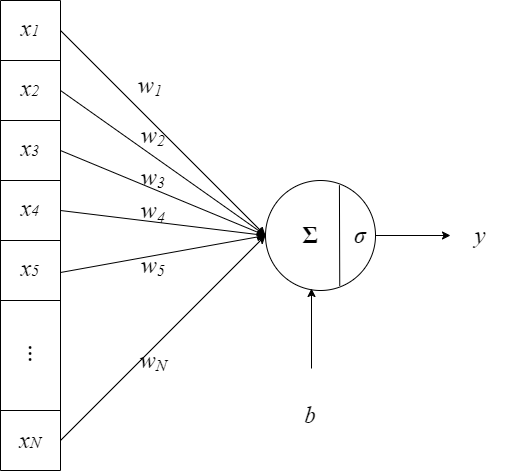
\includegraphics[width=0.5\linewidth]{figures/neuron.drawio.png}
    \caption{神經元示意圖}
    \label{fig:single-neuron}
\end{figure}

  其後羅氏(Rosenblatt)在 1958 年 \cite{rosenblatt_perceptron_1958} 提出感知器(Perceptron),本質上是結合數個神經元的運算,來實現更為複雜的函數功能。基於數學理論中的通用近似定理(Universal Approximation Theorm)\cite{funahashi_approximate_1989},感知器理想上可以近乎模擬一切函數。然而後續研究發現單層感知器具有線性不可分\footnote{例如無法貼合異或(Exclusive OR,XOR)運算等函數}的限制,於是出現了在輸入與輸出函數之間增加隱藏層(Hidden Layer)的多層感知器(Multi-layered Perceptron,MLP),由於在輸入與輸出之間的多層感知器可以藉助隱藏層的幫助實現函數的多次轉換,因而大大拓展了模型的適用範圍。此種計算模型由於是「加深隱藏層」得來的,因而被稱為深層類神經網路(Deep Neural Network)。
  
  然而,單純擁有能夠表達複雜函數的模型是不夠解決現實複雜的工程問題的。為了增加函數貼合的效率,魯氏(Rumelhart)與辛氏(Hinton)等人 \cite{rumelhart_learning_1986, rumelhart_learning_1987} 提出了反向傳播(Backpropagation)演算法,期望藉由計算輸出層與目標函數之間的誤差(Error),透過最佳化演算法計算出梯度(Gradient)後,經由隱藏層反向往輸入層,對整個類神經網路進行修正。於是配合圖形處理器平行運算的能力,資料中貼合函數的過程變得更有效率。如此透過深層類神經網路,找出資料輸入與輸出之間的函數關係的機器學習演算法,就稱之為深層學習(Deep Learning)。由於深層學習的可擴展性(Scalibility)與泛用性(Generalizability),不論在圖像、語音、文字等多個模態,深層類神經網路都已經獲得了廣泛應用,解決更加複雜的現實問題。

  實際上,根據資料特性的不同,並不是所有的資料都能單純的適用於這類輸入與輸出向量直接對應的模式,因此類神經網路又發展出不同的架構以適應資料本身的特性。前述的類神經網路由於運算過程單純是從輸入層經由多層感知器直接進行矩陣運算完成函數的模擬,因此被稱之為「前饋式類神經網路(Feed Forward Network,FFN)」。為了適應各種資料型態的特徵,藉由調整各神經元之間的連接關係,後續發展出了如卷積式(Convolutional)、遞迴式(Recurrent)與轉換器(Transformer)類神經網路等架構,以應對不同任務的需求。由於這些架構在語音與文字處理上相當常用,接下來將一一分別介紹:

\subsection{卷積式類神經網路}

  卷積式類神經網路(Convolutional Neural Network,CNN)為 1998 年由楊氏(LeCun) \cite{lecun_gradient-based_1998} 提出,旨在利用訊號處理上卷積(Convolution)的運算模擬人類視覺皮質感知 \cite{hubel_receptive_1959} 的特性,利用其移動不變性(Shift-invariance)來捕捉二維影像中的局部(Local)特徵,以便後續的類神經網路可以對輸入的資料進行更整體而全面的判斷。

\begin{figure}
    \centering
    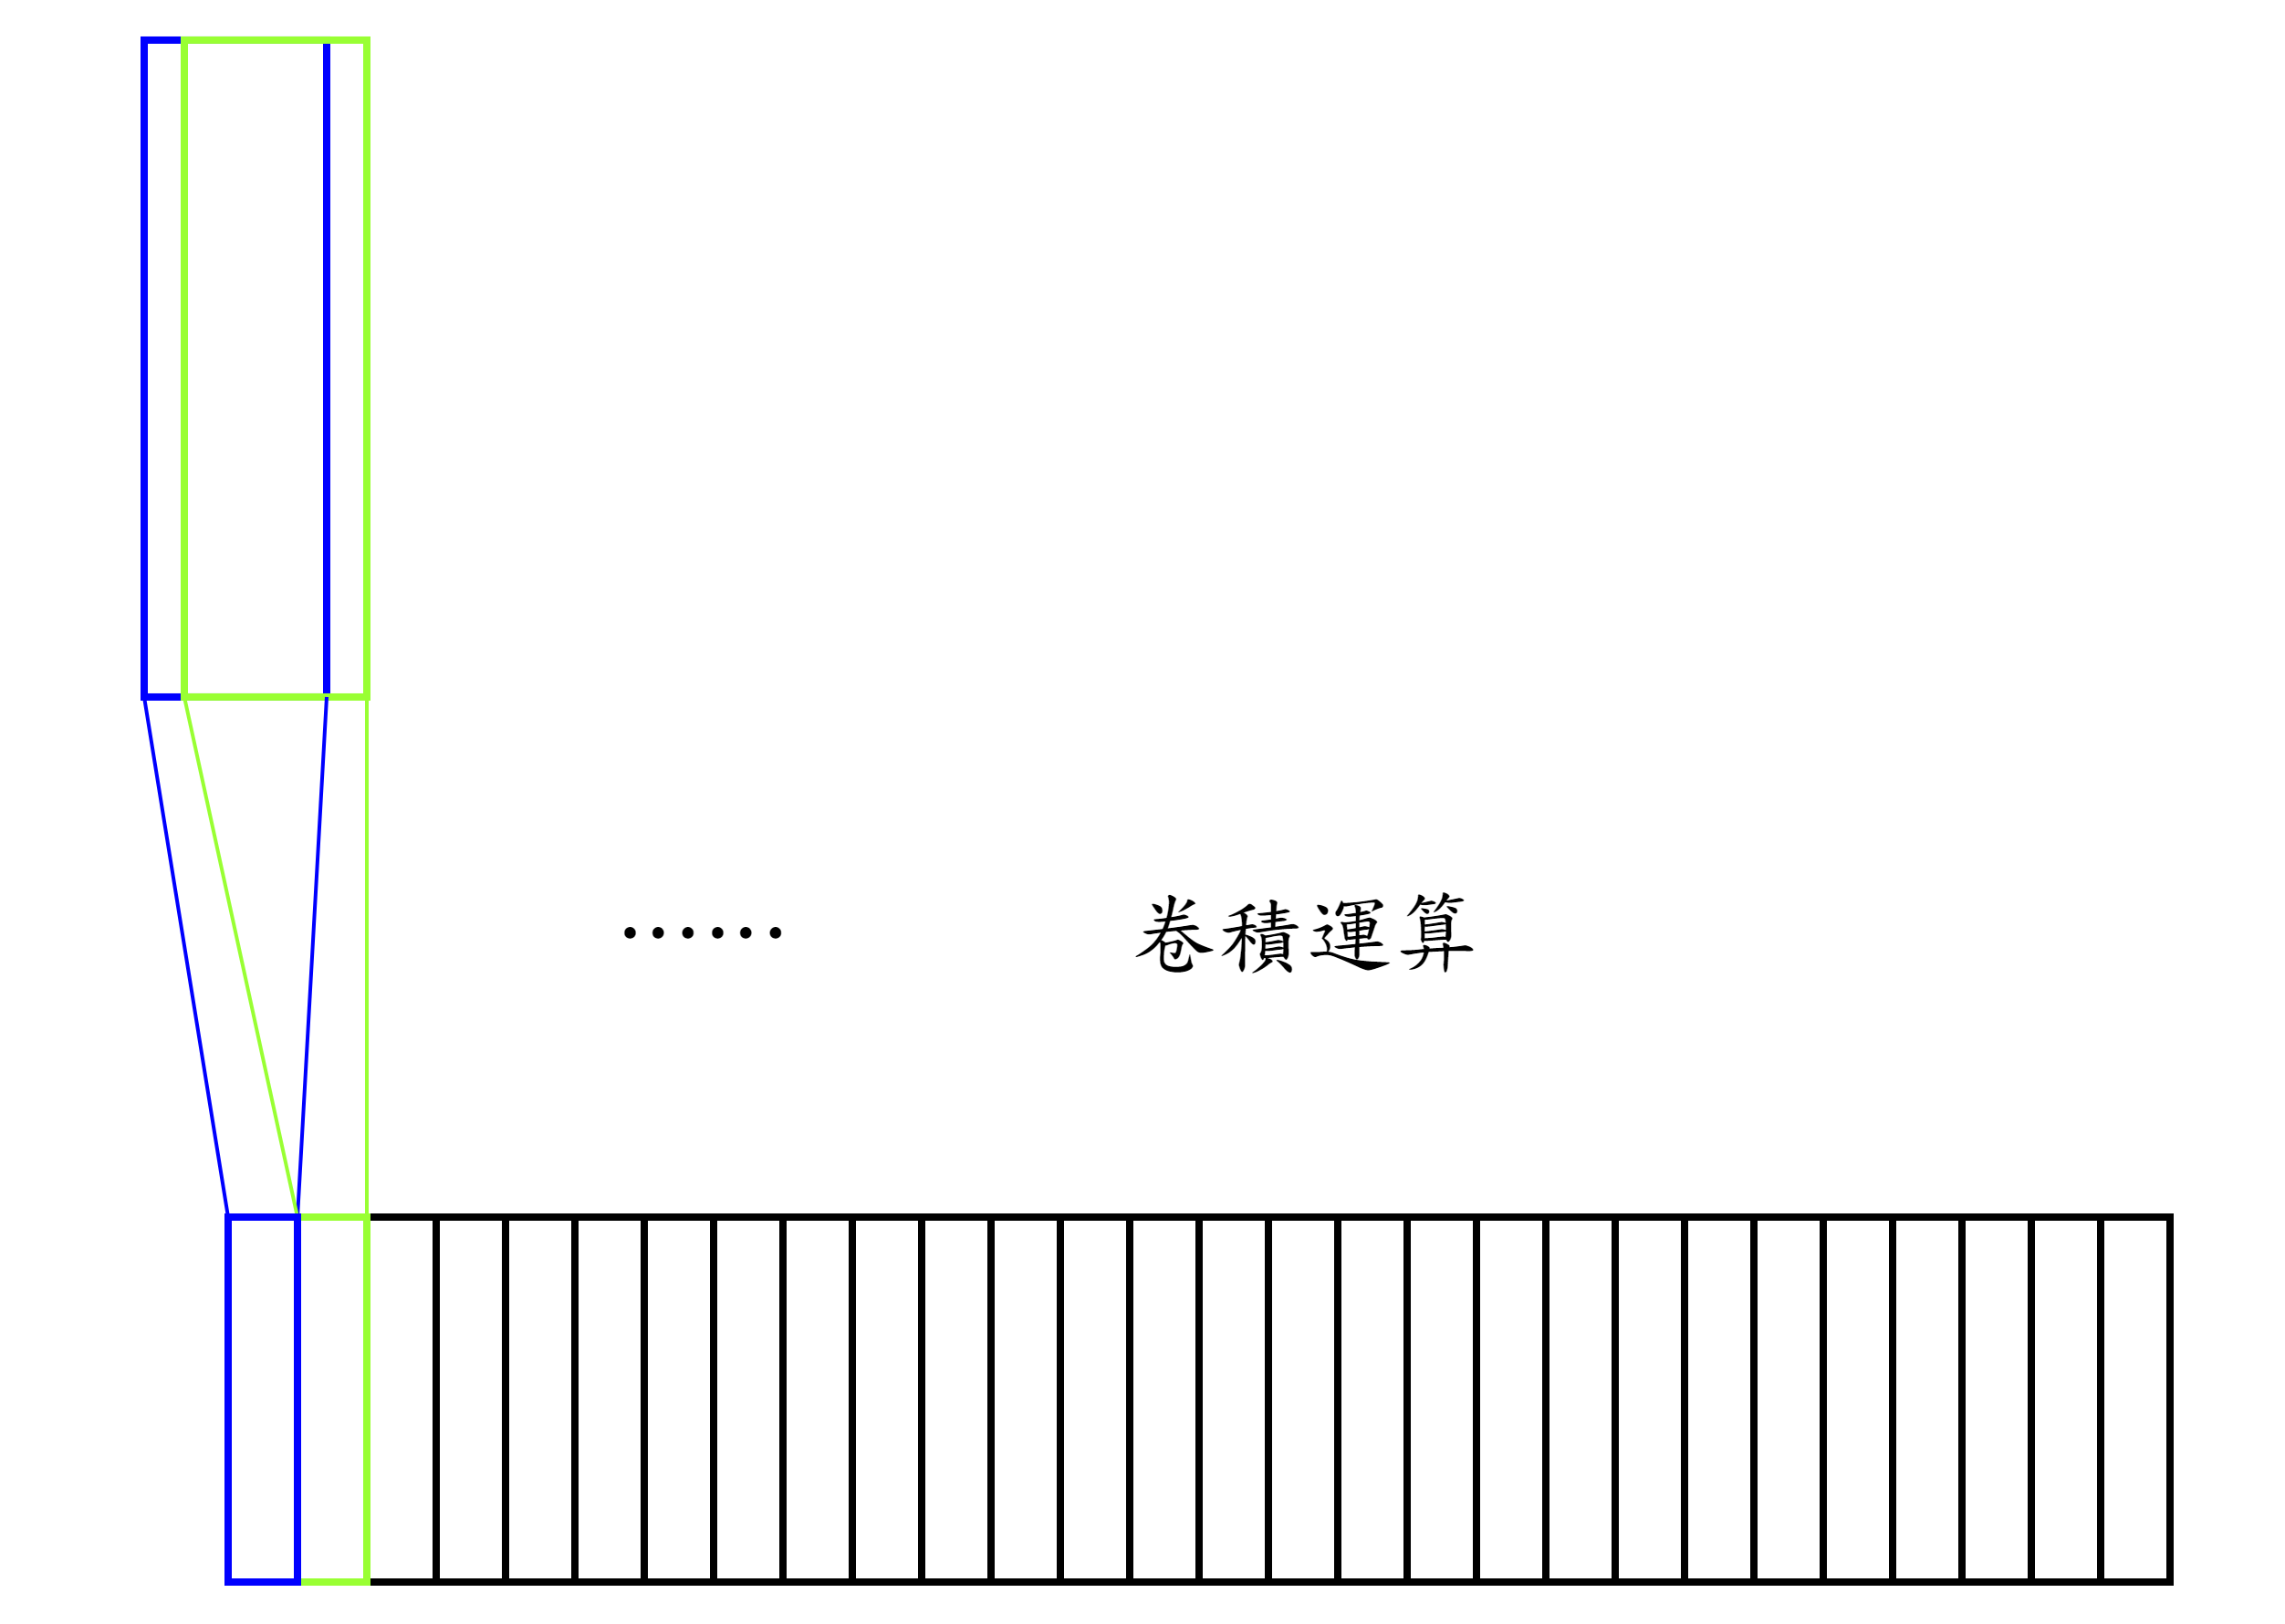
\includegraphics[width=0.5\linewidth]{figures/speechCNN.png}
    \caption{卷積神經網路作用於語音訊號示意圖}
    \label{fig:speech-cnn}
\end{figure}

  有別於圖像中經常是以像素 (Pixel)的三原色亮度進行卷積運算,在語音中卷積式類神經網路的處理對象,除了直接是空氣壓力波形的物理訊號以外,為了更方便機器模型判斷語音訊號的內容,透過聲學知識得到的聲學特徵或深層學習得出的語音表徵,也經常是語音處理中卷積層運算的對象。然而不論是何種輸入,有別於影像的二維資料,語音訊號的資訊是被呈現在時間軸的維度上,因此通常使用一維的卷積式類神經網路,以模仿人耳聽覺對時變訊號的窗框(Window)處理過程,讓模型可以觀察到輸入語音在不同解析度(Resolution)上的資訊,例如本研究特別著重的音位(Phoneme)等。

% // text embedding 先不寫

% // speech acoustic features 拖到後面去寫

\subsection{遞迴式類神經網路}

  不同於運算過程由輸入往輸出單向的前饋式和卷積式類神經網路,為了處理有記憶和狀態的資料,特別是會隨時間變化的序列資訊,在語音和文字的機器學習中,會將輸出訊號重新接回輸入層的遞迴式類神經網路(Recurrent Neural Network,RNN)是一個相當符合語言特性的選擇。此種網路以每個時間點(Timestep)為考慮對象,在每一步會對輸入層的向量進行運算後,不但將此結果算出一個輸出向量,還會得到另外一些數據保留作內部狀態,表示此前經歷過所有序列資料的記憶。常用的 遞迴式類神經網路類型有長短期記憶(Long Short-term Memory,LSTM)和閘門循環單元(Gated Recurrent Unit,GRU),示意圖與運算式分別如下:

%%%%%%%%%%


// 放運算式和示意圖

此類類神經網路通常會以下列介紹的序列至序列的形式被用在如語音辨識、語音合成或機器翻譯等和語言密切相關的任務中。

\subsection{序列至序列(Sequence-to-sequence,Seq2seq)模型}

由於許多以語言為主的資料經常以兩個序列互相配對的形式呈現,因此專門用以處理此類資料的模型被特別稱為序列至序列模型。此類模型一般的架構是由一個編碼器(Encoder)和一個解碼器(Decoder)構成,旨在模擬輸入與輸出序列之間的變化與相依關係(Dependency)。

此類模型一般有兩種模式:

其一是每個時間點都取得一個輸出的向量,用在輸入與輸出等長的任務之中,此模式又被稱為 token classification。

但更常見的狀況是,輸入與輸出兩者序列長度並不總是相同,此時典型的作法是,讓編碼器將輸入序列在每個時間點一一與模型進行運算,藉由內部表徵(Latent representation)的調整對整個輸入序列進行編碼,完成後將最後一個時間點的表徵作為整個序列的代表,此表徵向量會被稱為「語境向量(Context vector)」,接著被傳遞給解碼器依時序生成輸出訊號的序列。

\subsection{專注機制(Attention Mechanism)}

然而由於 RNN 本身需要編碼和解碼的資訊量是整個序列,對時間點距離比較遠的輸入容易被遺忘,也就是難以處理長期相依性(Long-term dependency)的問題。為解決這種困境,Luong 等人提出了「專注機制(Attention mechanism)」,讓解碼器除了依據語境向量的資訊以外,還可以對輸入序列的不同時間點分配權重,在生成輸出序列時重新從輸入序列中得到所需的訊息。

專注機制一般涉及三個向量之間的運算:query、key 和 value,其運算式如下:

(KQV 運算)

具有專注機制的序列至序列模型又被稱為 AED,透過專注機制的引入,大大改善了如語音辨識、機器翻譯等任務的效能。

\subsection{轉換器(Transformer)類神經網路}

儘管 RNN 本身善於處理時序資料,然而它難以平行化的架構限制卻大大束縛了其在訓練和推理(Inference)時的效率。由 attention 獲取靈感,2017 年瓦氏(Vaswani) 等人在 \_\_cite\_\_ 提出了一種完全由專注機制構成,不需依賴遞迴運算的序列至序列模型,用以解決最經典的機器翻譯任務。

\subsubsection{轉換器架構}

轉換器一樣沿用了 Attention 的 KQV 三組向量的邏輯,以 positional encoding 對序列中每個位置的時間點進行編碼,取代原先在 RNN 模型需要一一運算的過程,在實行平行計算的同時也能考慮到資料在不同時間點出現的效應。其整體架構如下:

(tfm 的圖)

(講多頭專注、KQV、FFN 那些)

由於轉換器不需對每個時間點一一運算,使其得以實現高度平行化的優勢,類神經網路得以透過專注機制的幫助同時進行序列資料的大量訓練,這種 scalibility 因而在自然語言和語音處理都獲得了巨大的進展,近乎取代了原先 RNN 的應用場景,近年甚至被電腦視覺的研究者推廣應用在圖像類的資料上( \_\_vit\_\_) ,足以展現此種模型架構的彈性與泛用性,是目前最前沿人工智慧的主流架構。

除了模型架構,機器學習中不可或缺的另一大 component 即是對資料的編碼過程。如何更有效率的讓機器可以理解、處理和輸出,是機器學習乃至深層學習的一大課題。面對捉摸不定、抽象且變化萬千的人類語言,語音和文字處理如何對資料去蕪存菁,表徵學習更是重中之重。


\section{表徵(Representation)學習與自監督式學習(SSL)}

為了讓機器可以理解輸入的資料,表徵學習是機器學習中不可或缺的一部分。
本節將從傳統機器學習用來處理語音的升學特徵開始,桌布介紹表語音表徵以及其學習過程的發展歷程。

\subsection{聲學特徵} 這邊直接跟下一個小姐合併



在語音處理中,在過往機器運算能力還沒有那麼強大的時候,人們基於聲學原理,使用 MFCC 為處理的對象。在文字中則通常使用 TF-IDF

(這邊寫 mfcc 的介紹)

\subsection{表徵學習}

後來 Mikolov 提出了 word2vec 的做法,使用 distributed representation 對文字的單詞(Word)進行編碼,透過大量的文本單詞之間的 co-occurence 去找出每個單詞最適合的語義表徵。其後 ELMo 提出了 contextualized embedding 的想法,更細緻的在單詞本身之外也嘗試對句子脈絡的語義進行詞嵌入(Word embedding)編碼。

\subsection{自監督學習}

爾後在 Transformer 模型被提出後,BERT (cite BERT) 被提出,從大量的文本與自專注機制之中,工程師們便可不借助人為的標記,透過預先設定的 pretext tasks 的引導,使得模型可以自己從大量文本中更細緻、更 contextualized 的自行找出語義關係,並在許多 NLP 的任務上獲得了 SoTA 的成績。自此「self-supervised learning (SSL)」的概念大行其道,這種以 pretext tasks 代替標註資料本身,從大量的未標註資料中利用資料本身結構進行學習的模式成為主流。由於其學習對象是發掘自大量的資料本身,可以更好的利用 NN 的泛化(Generalization)能力去找出什麼樣的資訊對於人們日常應用任務中是重要的並予以保留。

有鑑於文字處理方面的成功有許多的語音處理學者便嘗試將類似的模式套用在語音訊號之上自此提出了很多的語音基石模型而這些藉由語音基石模型得出來的語音表徵,也在很多任務上被證明可以超越傳統上使用的 fbank、 MFCC 等工程特徵,因為大量的語音資料庫本身可以幫助模型去萃取出更適用於各種語音任務上的向量表徵。

依照這些語音自監督模型的學習模式,大致可以分為重建式、預測式與對比式模型,以下分別按照這三類模式介紹這些語音基石模型:

(這邊接下來直接看以前碩論怎麼分。宏毅老師的 review paper 再說)\}

\subsubsection{重建式學習}

此類模型在文字處理以 BERT 為代表,BERT 本身屬於遮罩語言模型(Masked language model,MLM)。在語音中以 Mockingjay、TERA 為主要採取此模式的基石模型。

\subsubsection{預測式學習}

此類模型在文字處理以 GPT 為典型,不同於 BERT 是任意對資料進行擾動作為預訓練任務,這類模型的目標即是單純的自迴歸(Auto-regressive),可以用以下式子來表達其訓練 objective:

\[ \mbox{(寫那個 } y = p(x|x<t) \mbox{ 什麼的式子)} \]

在語音中以 APC 為代表。

(是不是有一個寫法把前兩個都當成預測,只是一個是重建一個是自迴歸?)

\subsubsection{對比式學習}

這類模型以 CPC 為主。在電腦視覺有 BYOL 等等。

\subsection{向量量化(Vector quantization)}這裡也跟下一個小節合併強調輸都累泊的部分



基於向量本身容易受噪聲擾動而導致訓練不穩定,因此為了穩定訓練,向量量化(Vector quantization)的技巧變常常為機器學習,尤其是語音這邊所使用。例如 vq-wav2vec 與其後的 wav2vec 2.0 就使用了這樣的技巧,HuBERT 本身對語音表徵進行 KMeans clustering 也是一個向量量化的手段。(是不是應該寫一下 KMeans 是什麼?)

(補說一下什麼是 discrete unit)

pseudo-label 

\subsection{離散單元與無文字(Textless)架構}

由於 HuBERT 本身的成功(好像要寫理由?),其後 Meta 提出了完全基於 HuBERT unit 的抽取方式,完全只依賴語音而不依靠文字標註的「無文字(Textless)」架構被提出,其代表作為 GSLM。(好像也要提一下 speech-to-speech 翻譯嗎?)

無文字目前在 QA (cite 實驗室的 DUAL) 跟語音到語音翻譯(Cite 並描述臺語翻英語翻譯)獲得了很好的成功。自此這類「離散單元(Discrete unit)」被視為一項類似文字卻不需要真的依賴人類文字標記的語音表徵,其最大優勢為儲存的 bit rate 低與可以套用 NLP 文字的「語言模型」之訓練模式。

然而,雖然在系統與應用 task 上獲得了很大的成功,但 unit 本身是否已經真的很好的可以替代文字,或能夠多少的幫助 spoken language model 的訓練與建立,仍然是目前本領域探討的焦點議題。有鑑於此,本論文基於語言知識,從最接近文字但又跟語音訊號最密切相關的 phoneme 開始探討,期望對 unit 本身究竟能夠帶給我們什麼特徵、如何幫助後續應用進行進一步的研究。

// 加入 speechtokenizer 嗎?


\section{本章節總結}

本章節先是對作為 building block 的類神經網路進行了基本原理的介紹,其後對本論文研究的核心 --- 「representation」與「discrete unit」的發展演進與歷史進行了簡單的梳理。此後兩章節就會緊扣著這些基石模型得到的離散特徵,將其與尤其是 phoneme 這類語音學標記之間的統計關係進行更進一步的分析。

(Ch 3 好像要講一下為什麼不做連續特徵 \& 為什麼要以 phoneme 為客體了 T\_T)


 

\chapter{單一語音離散表徵與語音標記的對應模式}

(Ch 3 好像要講一下為什麼不做連續特徵 \& 為什麼要以 phoneme 為客體了 T\_T) 
\section{動機簡介}  % \section{簡介}

由於 HuBERT 之後,unit 的使用很廣泛,因此為了研究 unit 本身為什麼會被如此適當的可以讓模型視為文字對語音資料進行訓練,我們先從離散表徵本身的特徵分析起。 

\section{相關研究}
近期已經有多項相關的研究,嘗試在 SSL 這麼厲害的表現之後找原因,因此有針對 unit 背後 repr 的特性進行分析的 work,例如 CITEUSPLEASE。 

\subsection{語音表徵的語音學分析}
在 HuBERT 出來之後,有一些研究像是 cite 等等,試圖探討對於語音表徵這樣語音模型的基礎進行各種從統計和語音學領域知識角度的分析,以期望能夠解釋為什麼模型可以擁有如此的表現。

此後,cite 等等作品則是從原先連續的表徵出發,開始往離散的量化向量,甚至是離散單元進行分析比對。雖然分析的切入角度可以相當多樣,例如 ABX、tsne 降維分群等等,但本次研究主要著重比對兩者之間在同一段語音序列上給予標籤的相關性,也就是以「偽標籤(pseudo-label)」的角度進行衡量。

\subsection{無文字(textless)語言模型}

這系列 textless 以 GSLM 為最主要代表作,旨在探討 unit 作為一種替代文字的方案。

本論文以 GSLM textless 採用的模型 units 為主要分析對象,企圖銜接兩者的脈絡,來佐證這些 unit 作為一種「類似或可替代文字的語音紀錄方式」在能夠發揮 LM 的特長背後,是否是基於符合語音學特徵帶來的,抑或有什麼其他特徵。


\subsection{以語音分段指標衡量對齊(Alignment)程度}
  
為了分析離散單元跟音位在語句序列之間的對齊程度,
本研究根據 \cite{strgar_phoneme_2023} 的方法
採用語音分段(Speech Segmentation)的標準去衡量。
具體動機為將被分到同一個離散單元編號的音框當成語音分段的同一類別的音位,
以此
期望可以
觀察出
在每一段語句中,
離散單元出現的順序與範圍,
與音位標註指示的範圍一致的程度。

%% alignment

\section{分析結果}
 
\subsection{基於各自音位的分析}

(放數據)

\subsection{基於語音學分類的分析}

(放數據)

\section{本章總結}


\chapter{多個語音離散表徵組合與語音標記間的關係}
\chapter{多個語音離散表徵組合與語音標記間的關係}

\section{動機}

基於單一語音單元表徵的限制,我們

放一些 rate 的東西


在现有的语音表征方法中,单一的离散单元虽然在许多任务中表现良好,但在处理长序列和时间分辨率方面存在局限性。Ren 等人的研究表明,许多相似的模式是以连续几个单元的形式出现的,这提示我们可以通过组合多个离散单元来更好地表示语音信号,从而提高模型在语音识别和语音翻译等任务中的性能 (\href{https://www.isca-archive.org/interspeech_2022/ren22_interspeech.html}{ISCA Archive}) (\href{https://deepai.org/publication/speech-pre-training-with-acoustic-piece}{DeepAI})。此外,SpeechTokenizer 的研究进一步展示了通过分层建模不同信息层次,能够在语音表示中捕捉到更丰富的语义和语音学信息 (\href{https://ar5iv.org/pdf/2308.16692}{ar5iv})。 


\section{相關研究}

\subsection{對語音離散表徵的分詞(tokenization)研究}

Ren 等人提出了使用声学片段(acoustic pieces)作为预训练的目标标签,通过对 HuBERT 代码进行句子片段化处理得到,能够显著改善自动语音识别(ASR)的性能 (\href{https://www.isca-archive.org/interspeech_2022/ren22_interspeech.html}{ISCA Archive})。Wu 等人介绍了 Wav2Seq,这是一种自监督方法,通过伪语言(pseudo languages)预训练编码器和解码器,显著提升了 ASR 和语音到文本翻译的性能 (\href{https://deepai.org/publication/speech-pre-training-with-acoustic-piece}{DeepAI})。

BEATs 提出了音频预训练方法,通过声学分片(acoustic tokenizers)学习音频离散表示,用于各种音频分类任务,表现出色 (\href{https://ar5iv.org/abs/2212.09058}{ar5iv})。

SpeechTokenizer 利用层级建模和语义蒸馏技术,通过多层残差量化器(RVQ)捕捉不同层次的信息,从而在语音表示中实现更高的语义和语音学特征保真度 (\href{https://ar5iv.org/pdf/2308.16692}{ar5iv})。





\section{分詞方法}


在文字語言模型上常用的分詞方法是 BPE,這種分詞方法比較於原本的 word 有幾個好處:

1 可以


 在文本处理中,常用的分词方法是 Byte Pair Encoding (BPE)。这种方法可以减少词汇表大小,提高模型的泛化能力,并能更好地处理罕见词和新词 (\href{https://deepai.org/publication/speech-pre-training-with-acoustic-piece}{DeepAI})。在语音处理中,类似的方法也可以用于离散语音单元的分词处理。例如,Ren 等人的方法通过句子片段化处理将高频代码模式合并为声学片段,从而有效地将输入音频与自然语言桥接起来 (\href{https://www.isca-archive.org/interspeech_2022/ren22_interspeech.html}{ISCA Archive}) (\href{https://deepai.org/publication/speech-pre-training-with-acoustic-piece}{DeepAI})。 


\paragraph{分词方法}

在文字语言模型上常用的分词方法是 Byte Pair Encoding (BPE)。这种分词方法相较于原本的单词表征有几个好处:

\begin{enumerate}
    \item \textbf{减少词汇表的大小}:提高模型的泛化能力。
    \item \textbf{处理罕见词和新词}:通过子词单元可以更好地处理罕见词和新词。
    \item \textbf{减少数据冗余}:提升训练和推理的效率。
\end{enumerate}
在语音处理中,类似的方法可以用于离散语音单元的分词处理。例如,Ren 等人的方法通过句子片段化处理(sentence piece)将高频代码模式合并为一个声学片段,从而有效地将输入音频与自然语言桥接起来 (\href{https://paperswithcode.com/paper/speech-pre-training-with-acoustic-piece}{Papers with Code})。

 


%%%%%%%%%%%%%%%%%%%
 

\section{衡量方式}

\subsection{字符(token)與音位之間的關係}




为了衡量离散单元和音位之间的关系,我们可以使用以下几个指标:

\begin{enumerate}
    \item \textbf{音位长条图(Phoneme Bar Chart)}:对单元进行频率统计,以了解每个单元在不同音位上的分布情况。
    \item \textbf{纯度(Purity)}:计算每个 cluster 单元内的音位纯度,以衡量单元对特定音位的代表性。 

\textbackslash{}Epz(j)[py∣z(y∗(j)∣j)]\textbackslash{}E\_{p\_z(j)\}\left[p\_{y|z\}(y\^*(j)|j) \textbackslash{}right]\textbackslash{}Epz(j)[py∣z(y∗(j)∣j)] 

以及每个音位对 cluster 的纯度,衡量音位在 cluster 中的一致性。
\textbackslash{}Epy(i)[pz∣y(z∗(i)∣i)]\textbackslash{}E\_{p\_y(i)\}\left[p\_{z|y\}(z\^*(i)|i) \textbackslash{}right]\textbackslash{}Epy(i)[pz∣y(z∗(i)∣i)]

    \item \textbf{熵(Entropy)和相互信息(Mutual Information, MI)}:从信息论角度探讨单元提供了多少背后音位的信息。 

I(y;z)H(y)=∑i∑jpyz(i,j)log⁡pyz(i,j)py(i)pz(j)∑ipy(i)log⁡py(i)\textbackslash{}frac\{I(y;z)\}{H(y)\}=\textbackslash{}cfrac\{\sum\_i \textbackslash{}sum\_j p\_{yz\}(i, j) \textbackslash{}log \textbackslash{}cfrac\{p\_{yz\}(i, j)\}{p\_y(i)p\_z(j)\}}\{\sum\_i p\_y(i) \textbackslash{}log p\_y(i)\}H(y)I(y;z)=∑ipy(i)logpy(i)∑i∑jpyz(i,j)logpy(i)pz(j)pyz(i,j) \textbackslash{}begin\{align\} \textbackslash{}frac\{I(y;z)\}{H(y)\}&=\textbackslash{}cfrac\{\sum\_i \textbackslash{}sum\_j p\_{yz\}(i, j) \textbackslash{}log \textbackslash{}cfrac\{p\_{yz\}(i, j)\}{p\_y(i)p\_z(j)\}}\{\sum\_i p\_y(i) \textbackslash{}log p\_y(i)\} \textbackslash{} \&=\textbackslash{}frac\{H(y)-H(y|z)\}{H(y)\} \textbackslash{} \&=1-\textbackslash{}frac\{H(y|z)\}{H(y)\} \textbackslash{}end\{align\}
\end{enumerate}

\subsection{壓縮比率}



\subparagraph{字符(token)与音位之间的关系}

为了衡量离散单元和音位之间的关系,我们可以使用以下几个指标:

\begin{enumerate}
    \item \textbf{音位长条图(Phoneme Bar Chart)}:对单元进行频率统计,以了解每个单元在不同音位上的分布情况。
    \item \textbf{纯度(Purity)}:计算每个 cluster 单元内的音位纯度,以衡量单元对特定音位的代表性。
    \item \textbf{熵(Entropy)和相互信息(Mutual Information, MI)}:从信息论角度探讨单元提供了多少背后音位的信息。
\end{enumerate}

\subparagraph{压缩比率}

通过对离散单元进行分词和压缩,可以显著减少序列长度,从而提高训练和推理的效率。我们可以通过计算压缩比率来衡量这种方法的有效性。

 


\section{分析結果}


\subsection{基於各自音位的分析}

在此部分,我们将展示基于音位的频率统计结果和纯度分析结果。通过这些分析,我们可以了解离散单元在捕捉音位特征方面的表现 (\href{https://www.isca-archive.org/interspeech_2022/ren22_interspeech.html}{ISCA Archive}) (\href{https://deepai.org/publication/speech-pre-training-with-acoustic-piece}{DeepAI})。

\subsection{基於語音學分類的分析}


在此部分,我们将展示基于语音学分类的分析结果。这包括对离散单元在不同语音学类别(如元音、辅音)中的表现分析,以评估其在不同语音特征下的表现 (\href{https://www.isca-archive.org/interspeech_2022/ren22_interspeech.html}{ISCA Archive}) (\href{https://deepai.org/publication/speech-pre-training-with-acoustic-piece}{DeepAI})。



 
\section{應用在語音任務的實驗}

\subsection{語音辨識}

\subsubsection{實驗設定與資料集}

\subsubsection{實驗結果與其和分析數據間的關係}



\section{本章總結}

总结本章的内容,回顾离散单元在多个语音表征组合中的应用和优势,并展望未来的研究方向。


\section{分詞方法}

在文字語言模型上常用的分詞方法是 BPE,這種分詞方法比較於原本的 word 有幾個好處:

1 可以



\section{衡量方式}

\subsection{字符(token)與音位之間的關係}

\subsection{壓縮比率}




\section{分析結果}

\subsection{基於各自音位的分析}

\subsection{基於語音學分類的分析}



\newpage



\section{應用在語音任務的實驗}

\subsection{語音辨識}

\subsubsection{實驗設定與資料集}

\subsubsection{實驗結果與其和分析數據間的關係}



\section{本章總結}

